\documentclass{article}
\usepackage{graphicx}
\newcount\ContadorDFigs\ContadorDFigs=0
\def\NumDFig{
\global\advance\ContadorDFigs by 1
Figura \the\ContadorDFigs\ $\,$
}
\begin{document}
\section{Planif\/icaci\'on de procesos}
Cuando hay m\'as de un proceso ejecutable, el sistema operativo 
debe decidir cu\'al ejecutar\'a primero. La parte del sistema operativo 
que toma esta decisi\'on se denomina {\bf planif\/icador}: el algoritmo 
que usa se denomina {\bf algoritmo de planif\/icaci\'on}.

Para asegurarse de que ning\'un proceso se ejecute durante demasiado 
tiempo, casi todas las computadoras tienen incorporado un cron\'ometro 
o reloj electr\'onico que genera interrupciones periodicamente. Es com\'un 
que la frecuencia sea de 50 o 60 interrupciones por segundo, pero en muchas 
computadoras el sistema operativo puede ajustar la frecuencia del cron\'ometro 
al valor que desee. En cada interrupci\'on de reloj, el sistema operativo se 
ejecuta y decide si debe permitirse que el proceso que se est\'a ejecutando 
actualmente contin\'ue o si ya disfrut\'o de suf\/iciente tiempo de CPU por 
el momento y debe suspenderse para otorgar a otro proceso la CPU.

La estrategia de permitir que procesos l\'ogicamente ejecutables se 
suspendan temporalmente se denomina {\bf planif\/icaci\'on expropiativa} o 
{\bf planif\/icaci\'on apropiativa} en contraste con el m\'etodo de 
{\bf ejecuci\'on hasta terminar} (o {RTC: Run To Completion}) de los 
primeros sistemas por lotes. La ejecuci\'on hasta terminar (RTC) se 
denomina {\bf planif\/icaci\'on no expropiativa}. El hecho de que un proceso 
pueda ser suspendido en un instante arbitrario, sin advertencia, para que 
otro proceso pueda ejecutarse, da lugar a {\bf condiciones de competencia} y 
requiere sem\'aforos, monitores\footnote{Una primitiva de sincronizaci\'on 
propuesta en la decada de los 70s del siglo pasado, v\'ease \cite{Tanenbaum}, 
p\'agina 69}, mensajes o alg\'un otro m\'etodo avanzado para prevenirlas.  

Se examinar\'an algunos algoritmos de planif\/icaci\'on espec\'if\/icos.

\subsection{Planif\/icaci\'on {\it round robin} (de torneo)}
Uno de los algoritmos de planif\/icaci\'on m\'as antiguos, sencillos, equitativos 
y ampliamente utilizados es el de {\bf round robin}. A cada proceso se le 
asigna un intervalo de tiempo, llamado {\bf cuanto}, durante el cual se le 
permite ejecutarse. Si el proceso aun se est\'a ejecutando al expirar su 
cuanto, el sistema operativo se apropia de la CPU y se la da a otro proceso. 
Si el proceso se bloquea, el sistema operativo asigna la CPU a otro proceso. 
Si el proceso termina antes de expirar el cuanto, naturalmente la CPU tambi\'en 
se conmuta. El {\it round robin} es facil de implementar. Todo lo que el 
planif\/icador tiene que hacer es mantener una lista de procesos ejecutables como 
se muestra en las f\/iguras siguientes:
%\begin{figure}[h]
%\begin{center}
%\includegraphics[scale=0.075]{img/Figura2_22Tanenbaum.jpg}
%\caption{Planif\/icaci\'on round robin}
%\label{ValvanoVol3Pag176}
%\end{center}
%\end{figure}
$$
\begin{array}{c}
\begin{array}{cc}
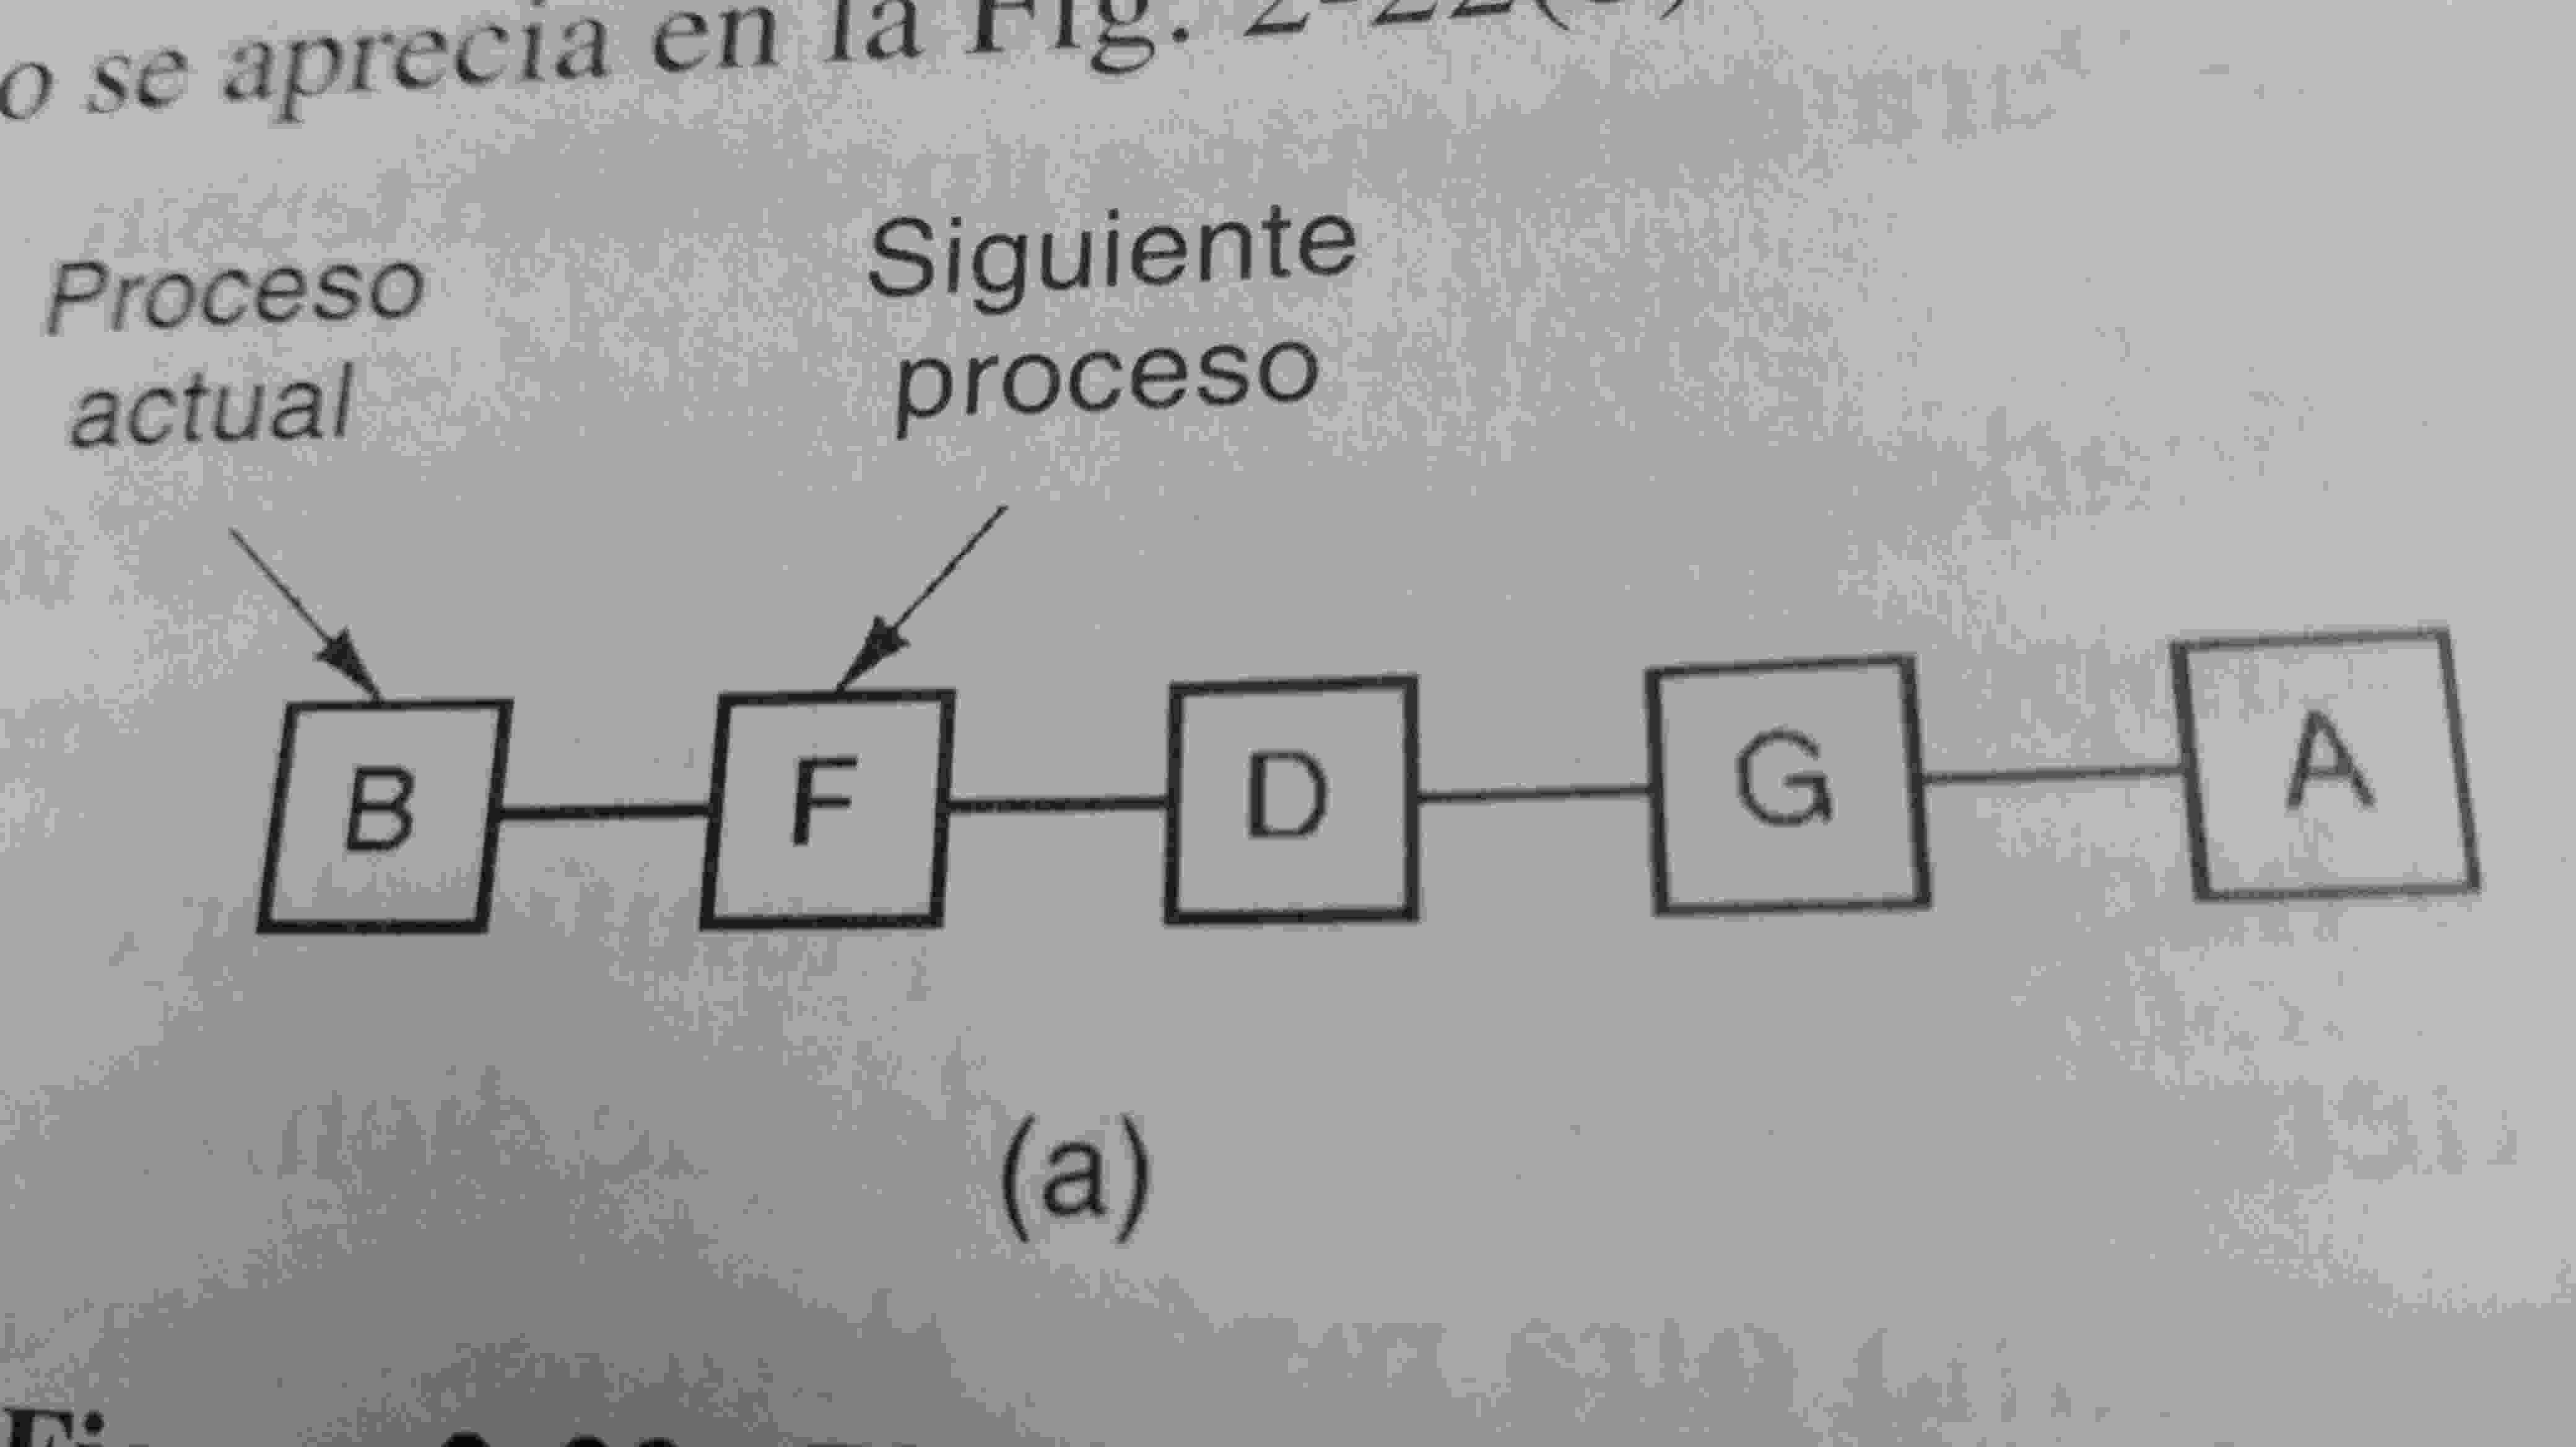
\includegraphics[scale=0.04]{img/Figura2_22TanenbaumA.jpg}&
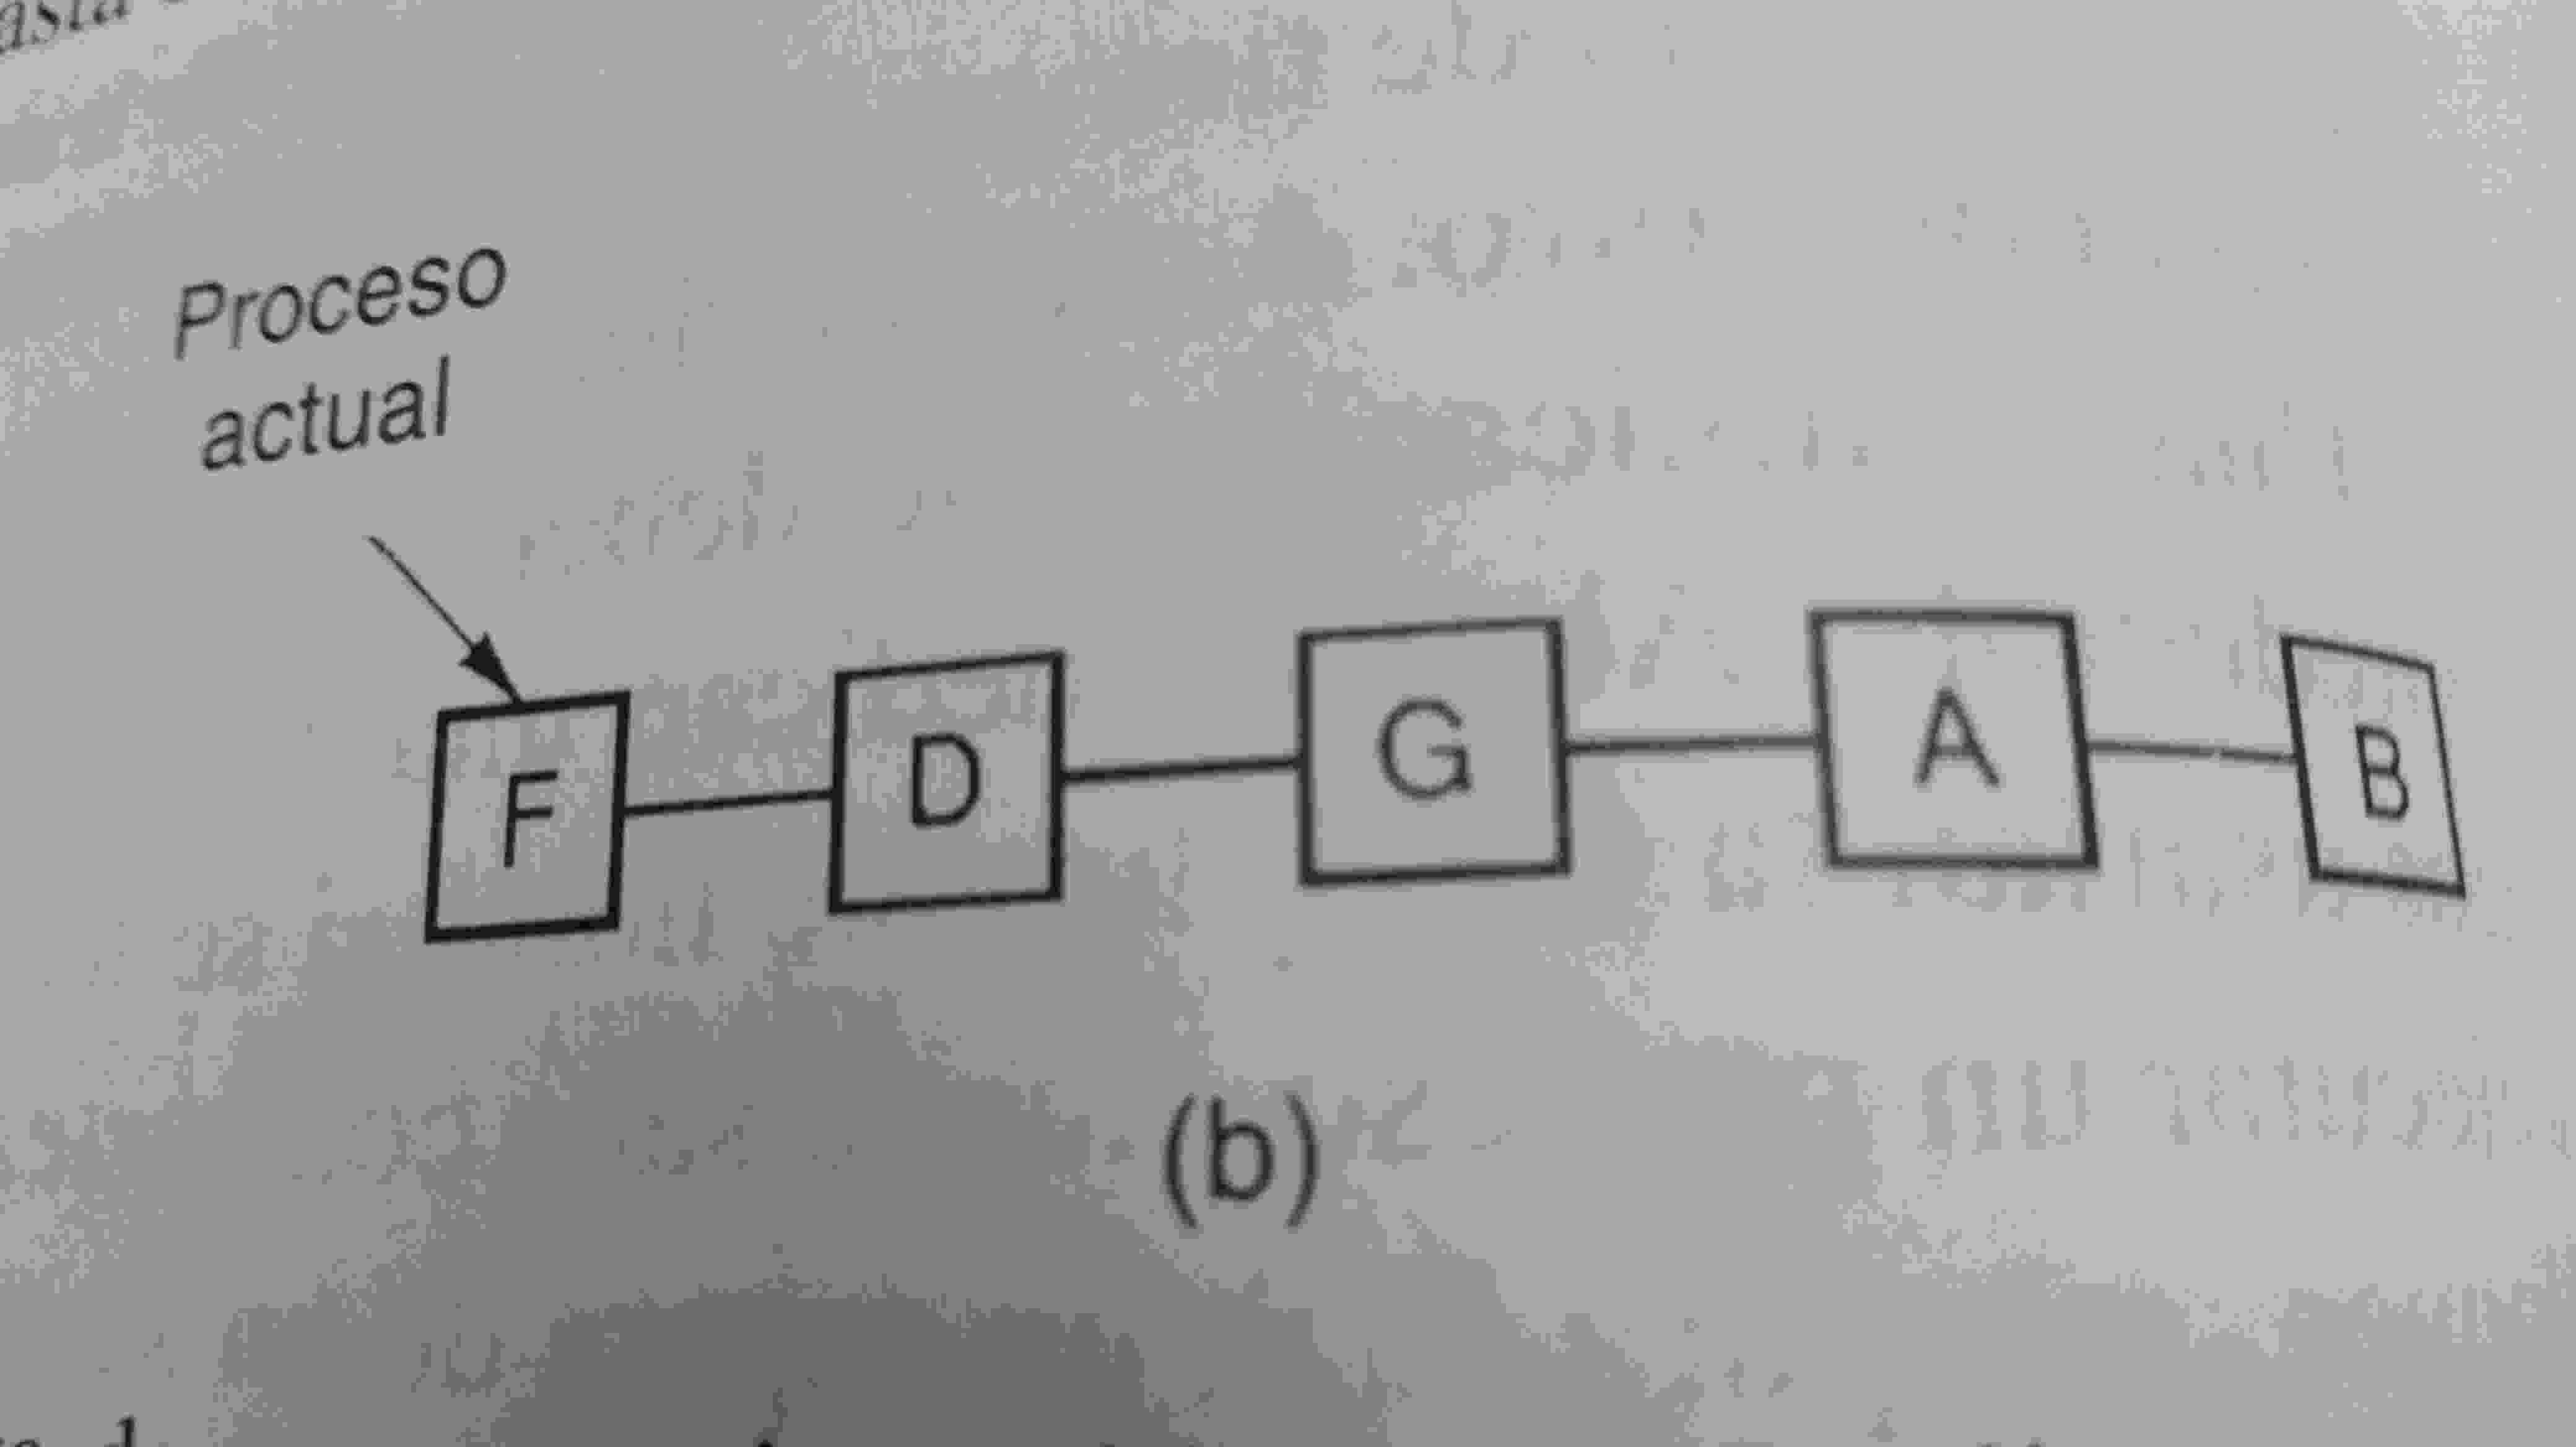
\includegraphics[scale=0.04]{img/Figura2_22TanenbaumB.jpg}
\end{array}\\
\mbox{\NumDFig\ Planif\/icaci\'on {\it round robin}}
\end{array}
\label{Fig2_22Tanenbaum}
$$
Cuando un proceso gasta su cuanto se le coloca al f\/inal de la lista como se muestra 
en la f\/igura de la derecha. El punto clave en el planif\/icador round robin es la 
duraci\'on del cuanto. La conmutaci\'on de un proceso a otro requiere cierto tiempo 
para llevar a cabo las tareas administrativas: guardar y cargar registros y mapas de 
memoria, actualizar diversas tablas y listas, etc. Su\-pon\-ga\-mos que esta 
{\bf conmutaci\'on de proceso} o {\bf cambio de contexto} requiere 5 ms. Supongamos 
tambi\'en que usamos cuantos de 20 ms. Con estos par\'ametros, despu\'es de realizar 
trabajo util durante 20 ms, la CPU tendr\'a que ocupar 5 ms en la conmutaci\'on de 
procesos. Se desperdiciar\'a el 20\% del tiempo de CPU en gastos extra administrativos. 
Como alternativa, podr\'ian usarse cuantos de 500 ms, ahora el tiempo de ``gasto'' 
administrativo es aproximadamente del 1\%, pero esto tambi\'en puede acarrear 
situaciones adversas. Considere un sistema de tiempo compartido con 10 usuarios 
interactivos que pulsan la tecla de retorno de carro aproximadamente al mismo tiempo: 
diez procesos se pondr\'ian en la lista de procesos ejecutables. Si la CPU est\'a ociosa, 
el primero se iniciar\'a de inmediato, el sgundo podr\'ia no iniciarse hasta cerca de 
medio segundo despu\'es, y as\'i sucesivamente. El proceso que le haya tocado ser 
\'ultimo podr\'ia tener que esperar 5 segundos antes de tener su oportunidad. Para 
casi cualquier usuario, un retardo de 5 segundos en la respuesta a un comando corto 
ser\'ia terrible. El mismo problema puede presentarse en una computadora personal 
que maneja multiprogramaci\'on.

En conclusi\'on: escoger un cuanto demasiado corto causa demasiados cambios de 
contexto (conmutaciones de proceso) y reduce la ef\/iciencia de la CPU, pero escogerlo 
demasiado largo puede dar pie a una respuesta def\/iciente a solicitudes interactivas. 
un cuanto de 100 ms suele ser un t\'ermino medio razonable.

La planif\/icaci\'on en {\it round robin} supone impl\'icitamente que todos los 
procesos son igualmente importantes. Con fecuencia, las personas que poseen y operan 
sistemas de computadora consideran que algunos procesos deben ser considerados 
como m\'as importantes que otros. En una computadora militar, los procesos iniciados 
por generales podr\'ian iniciar con prioridad 100, los iniciados por coroneles con 90, 
por mayores con 80, por capitanes con 70, por tenientes con 60, etc.  Incluso en una 
PC con un solo usuario, puede haber m\'ultiples procesos, algunos m\'as importantes 
que otros. Por ejemplo, un proceso demonio que env\'ia correo electr\'onico en segundo 
plano debe tener menor prioridad que un proceso que est\'a exhibiendo video en tiempo 
real en la pantalla. La necesidad de tener en cuenta factores externos da origen a la 
{\bf planif\/icaci\'on por prioridad}. 

\subsection{Planif\/icaci\'on por prioridad}
La idea b\'asica es sencilla: a cada proceso se le asigna una prioridad, y se permite 
que se ejecute el proceso ejecutable que tenga la prioridad m\'as alta. Las prioridades 
se pueden asignar est\'atica o din\'amicamente.A f\/in de evitar que los procesos de 
alta prioridad se ejecuten indef\/inidamente, el planif\/icador puede 
reducir la prioridad de los procesos que actualmente se ejecutan en cada tic del 
reloj (esto es, en cada interrupci\'on de reloj). Si esta acci\'on hace que la 
prioridad se vuelva menor que la de otro proceso, ocurrir\'a una conmutaci\'on de 
procesos. Como alternativa, se podr\'ia asignar a cada proceso un cuanto m\'aximo en 
el que se le permitiera tener la CPU continuamente; cuando se agota este cuanto, se da 
oportunidad al proceso con la siguiente prioridad m\'as alta de ejecutarse.

Tambi\'en puede asignarse prioridades din\'amicamente a f\/in de lograr ciertos objetivos 
del sistema. Por ejemplo, algunos procesos est\'an limitados para seguir avanzando 
principalmente debido a E/S y pasan la mayor parte del tiempo esperando que terminen 
operaciones de E/S, siempre que uno de estos procesos necesite la CPU, se le deber\'a 
otorgar de inmediato, con objeto de que pueda iniciar su siguiente solicitud de E/S, 
que entonces podr\'a proceder en paralelo con otro proceso que s\'i est\'a realizando 
c\'alculos. Si hici\'eramos que los procesos limitados por E/S esperaran mucho tiempo 
la CPU, implicar\'ia tenerlos por ah\'i ocupando memoria duarnte un tiempo 
innecesariamente largo. Un algoritmo sencillo para dar buen servicio a los procesos 
limitados por E/S es asignarles la prioridad $1/f$, donde $f$ es la fracci\'on del 
\'ultimo cuanto que un proceso utiliz\'o. Un proceso que us\'o solo 2 ms de su cuanto 
de 100 ms recibir\'ia una prioridad de 50, en tanto que un proceso que se ejecut\'o 
50 ms antes de bloquearse obtendr\'ia una prioridad de 2, y uno que ocup\'o todo su 
cuanto obtendr\'ia una prioridad de 1.

En muchos casos es conveniente agrupar los procesos en clases de prioridad y usar 
planif\/icaci\'on por prioridad entre las clases pero planif\/icaci\'on {\it round 
robin} dentro de cada clase. Por ejemplo, en un sistema con 4 clases de prioridad 
con prioridades 1, 2, 3, 4 respectivamente, el algoritmo de planif\/icaci\'on es el 
siguiente: en tanto haya procesos ejecutables en la clase de prioridad 4, se 
ejecutar\'a cada uno durante un cuanto, con round robin, sin ocuparse de las 
clases de menor prioridad. Si la clase de prioridad 4 est\'a vacia, se ejecutan 
los procesos de clase 3 con round robin. Si tanto la clase 4 como la 3 est\'an 
vacias, se ejecutar\'an los procesos de la clase 2 con round robin, etc. 
Ocasionalmente se ajustar\'an las prioridades de las clases para que las clases 
de baja prioridad no mueran de inanici\'on.

\subsection{Colas m\'ultiples}
\subsection{El primer trabajo m\'as corto/Primero el trabajo m\'as corto}
\subsection{Planif\/icaci\'on garantizada}
\subsection{Planif\/icaci\'on por loter\'ia}
\subsection{Planif\/icaci\'on en tiempo real}
Un sistema de {\bf tiempo real} es uno en el que el tiempo desempe\~na 
un papel esencial. Por lo regular, uno o m\'as dispositivos externos a la 
computadora generan est\'imulos, y la computadora debe reaccionar a ellos 
de la forma apropiada dentro de un plazo f\/ijo. Por ejemplo, la computadora 
de un reproductor de discos compactos recibe los bits conforme salen de 
la unidad de disco y los debe convertir en m\'usica dentro de un intervalo 
de tiempo muy estricto. Si el c\'alculo toma demasiado tiempo la m\'usica 
sonar\'a raro. Otros sistemas de tiempo real son los de monitoreo de 
pacientes en las unidades de cuidado intensivo de los hospitales, el 
pil\'oto autom\'atico de un avi\'on y los controles de seguridad de un 
reactor nuclear. En todos estos casos, obtener la respuesta correcta 
pero demasiado tarde suele ser tan malo como no obtenerla.

Los sistemas de tiempo real generalmente de clasif\/ican como de {\bf tiempo 
real estricto}, lo que signif\/ica que hay plazos absolutos que deben cumplirse 
a como de lugar, y {\bf tiempo real flexible}, lo que signif\/ica que es tolerable 
no cumplir ocasionalmente con un plazo. En ambos casos, el comportamiento de 
tiempo real se logra dividiendo el programa en varios procesos, cada uno de 
los cuales tiene un comportamiento predecible y conocido por adelantado. 
Estos procesos generalmente son de corta duraci\'on y pueden ejecutarse hasta 
terminar en menos de un segundo. Cuando se detecta un suceso externo, el 
planif\/icador debe programar los procesos de modo tal que se cumplan todos los 
plazos. 

Los sucesos a los que puede tener que responder un sistema de tiempo real 
pueden clasif\/icarse tambi\'en como {\bf peri\'odicos} (que ocurren a intervalos 
regulares) o {\bf aperi\'odicos} (que ocurren de forma impredecible). Es posible 
que un sistema tenga que responder a m\'ultiples corrientes de eventos 
periodicos. Dependiendo de cu\'anto tiempo requiere cada suceso por separado, 
tal vez ni siquiera sea posible manejarlos todos. por ejemplo, si hay $m$ 
eventos periodicos y el evento $i$ ocurre con el periodo $P_{i}$ y requiere 
$C_{i}$ segundos de tiempo de CPU para ser manejado, la carga solo puede 
manejarse si
$$
\sum_{i=0}^{m}\frac{C_{i}}{P_{i}}\leq 1
$$
Un sistema de tiempo real que satisface este criterio es {\bf planif\/icable}.

Por ejemplo, consideremos un sistema de tiempo real flexible con tres 
sucesos periodicos, con periodos de 100, 200 y 500 ms respectivamente. Si estos 
eventos requieren 50, 30 y 100 ms detiempo de CPU por evento, respectivamente, 
el sistema es planif\/icable porque 
$$
\frac{50}{100}+\frac{30}{200}+\frac{100}{500}=0.5+0.15+0.2=0.85<1
$$
Si se agrega un cuarto evento con un periodo de 1 s, el sistema seguir\'a 
siendo planif\/icable en tanto que este evento no necesite m\'as de 150 ms de 
tiempo de CPU por evento. Un supuesto impl\'icito en este c\'alculo es que el 
gasto extra del cambio de contexto es tan peque\~no que puede ignorarse.


Pag. 91 \cite{Tanenbaum}, sistemas operativos disenio e implementacion.

\begin{thebibliography}{9}
\bibitem{Tanenbaum}Andrew S. Tanenbaum, ``Sistemas Operativos, 
Dise\~no e Implementaci\'on,'' Editorial Pearson, 2002.
\end{thebibliography}
\end{document}
